Wybrane logo mBanku ma kształt prostokątny, złożone jest z:
\begin{itemize}
    \item pionowych pasów koloru: czerwonego, żółtego, zielonego, czarnego, niebieskiego;
    \item umieszczonego na nich białego napisu \emph{mBank}.
\end{itemize}

Jako najbardziej charakterystyczne cechy obrazu wybrane zostały trzy kolorowe pasy o największej powierzchni - czerwony, żółty i zielony. Ich bliskie siebie położenie oraz względnie niepowtarzalny kształt związany z nachodzeniem na nie białego napisu będą przydatne na etapie dalszego przetwarzania i ich wykrywania.

% \begin{figure}[H]
% \centering
% \begin{minipage}{.4\textwidth}
%   \centering
%   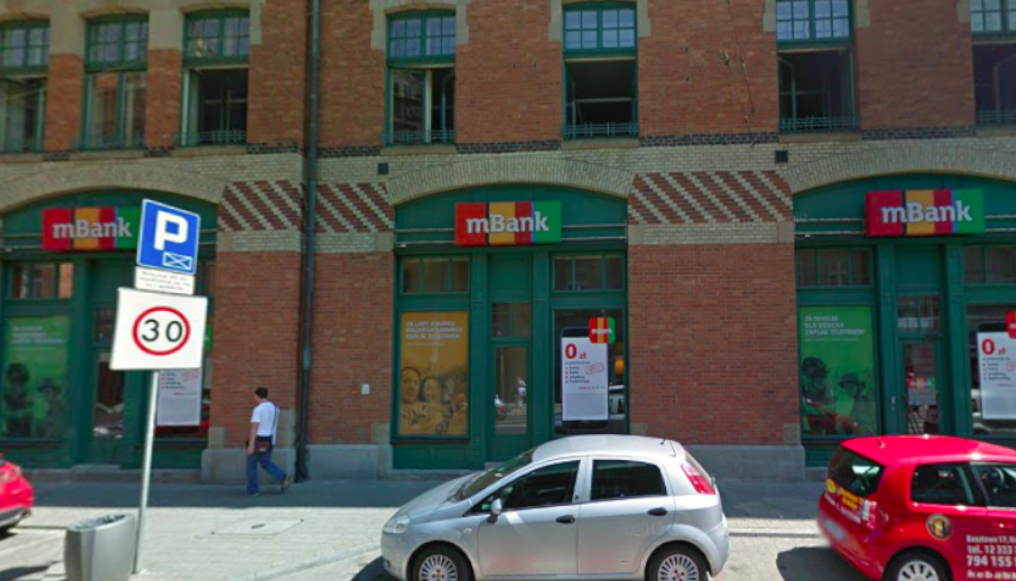
\includegraphics[width=\linewidth]{figures/img1.png}
%   \captionof{figure}{Wykres funkcji Rastrigina}
%   \label{fig:rastrigin}
% \end{minipage}%
% \begin{minipage}{.4\textwidth}
%   \centering
%   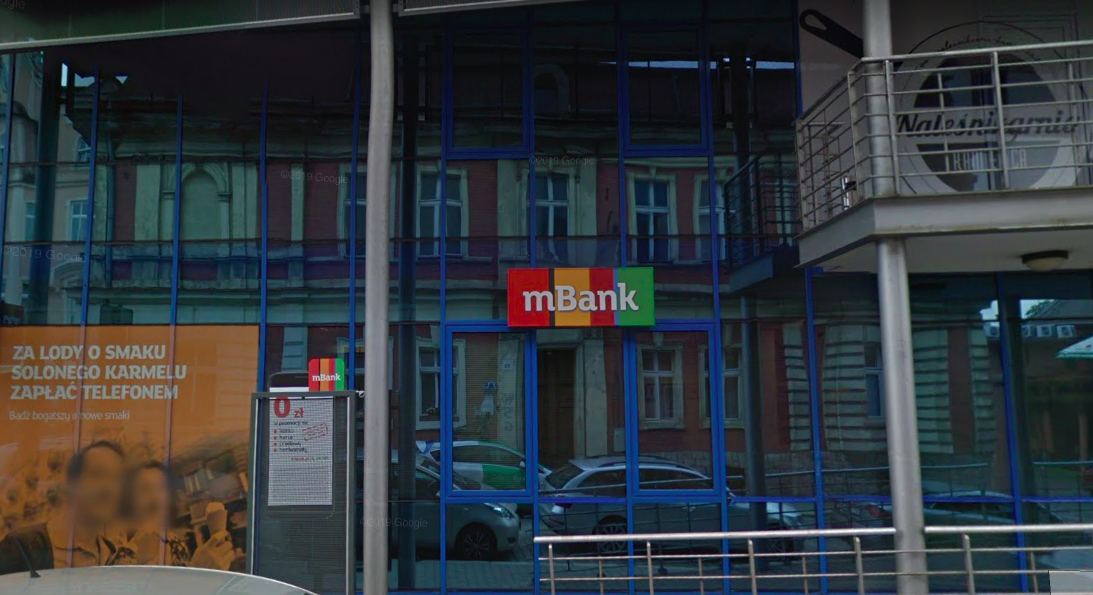
\includegraphics[width=\linewidth]{figures/img2.png}
%   \captionof{figure}{Wykres funkcji Schwefela}
%   \label{fig:schwefel}
% \end{minipage}
% \end{figure}

\begin{figure}[h]
\begin{subfigure}{.5\textwidth}
  \centering
  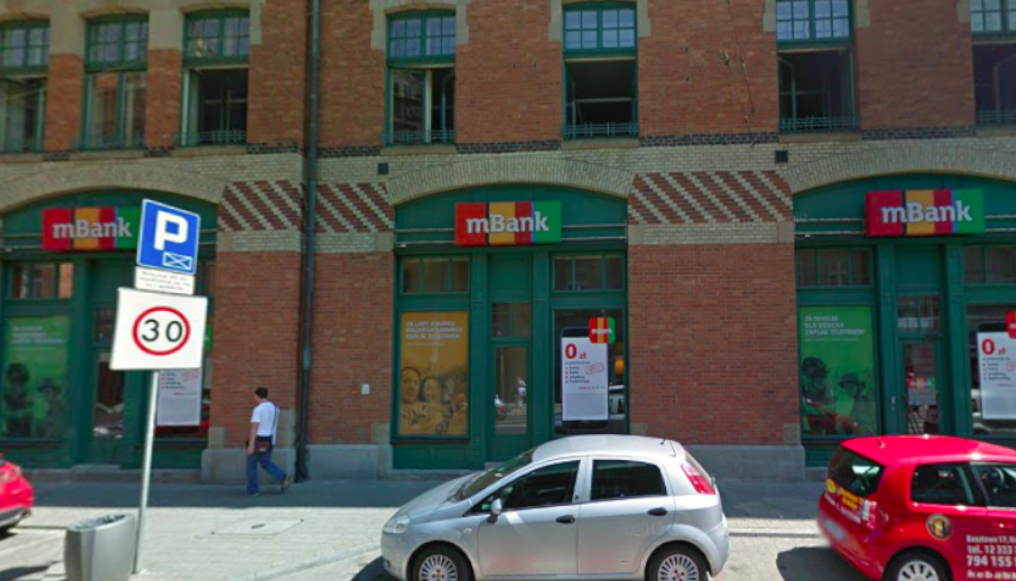
\includegraphics[width=.8\linewidth]{figures/img1.png}
  \caption{Obraz a}
  \label{fig:sfig1}
\end{subfigure}%
\begin{subfigure}{.5\textwidth}
  \centering
  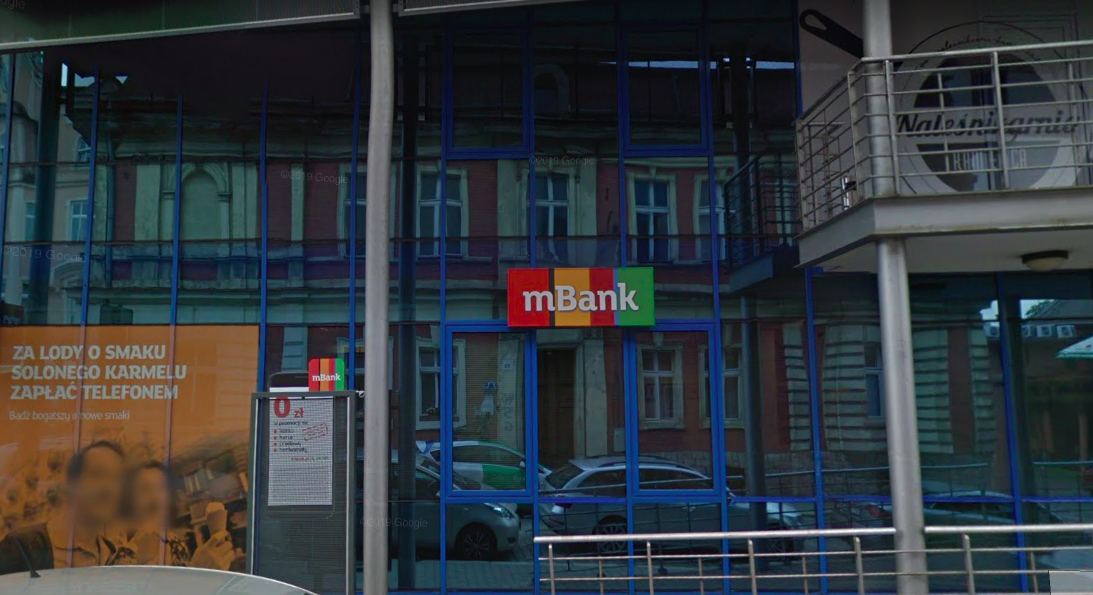
\includegraphics[width=.8\linewidth]{figures/img2.png}
  \caption{Obraz b}
  \label{fig:sfig2}
\end{subfigure}
\begin{subfigure}{.5\textwidth}
  \centering
  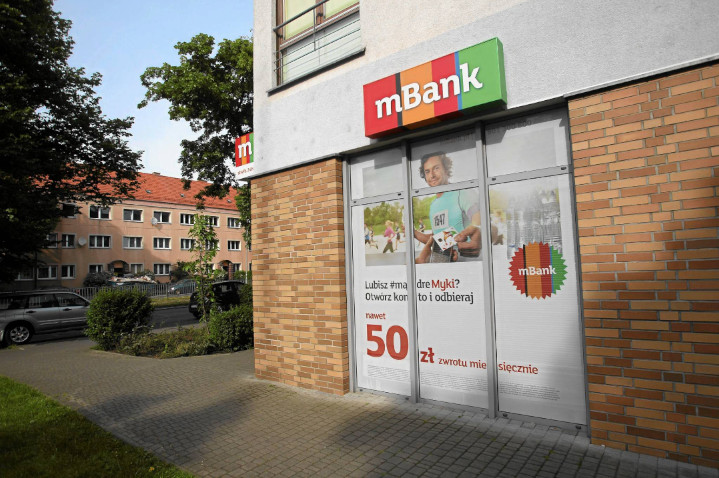
\includegraphics[width=.8\linewidth]{figures/img3.png}
  \caption{Obraz c}
  \label{fig:sfig2}
\end{subfigure}
\begin{subfigure}{.5\textwidth}
  \centering
  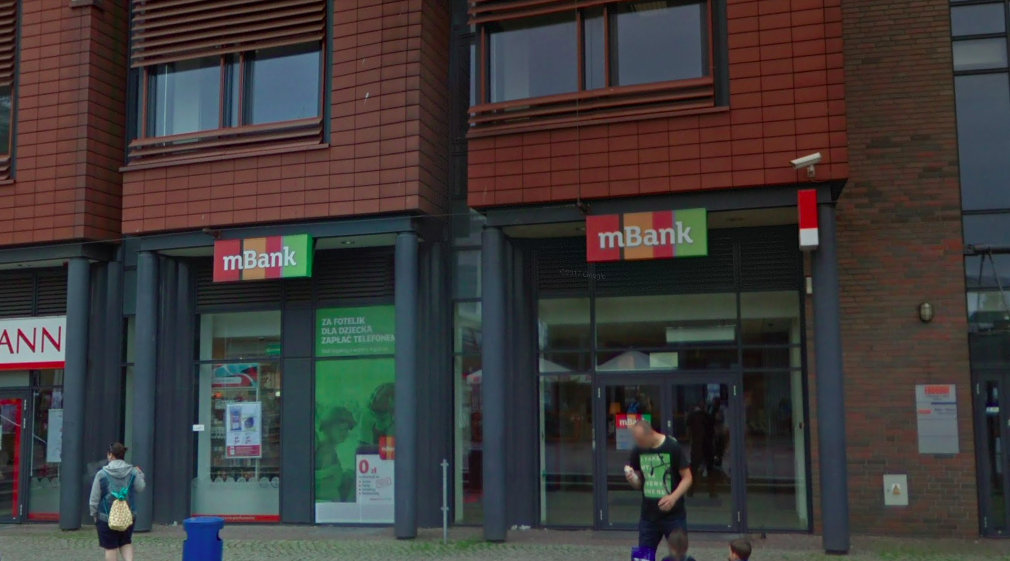
\includegraphics[width=.8\linewidth]{figures/img4.png}
  \caption{Obraz d}
  \label{fig:source-photos}
\end{subfigure}
\caption{Wybrane obrazy wejściowe}
\end{figure}